%%%%%%%%%%%%%%%%%%%%%%%%%%%%%%%%%%%%%%%%%%%%%%%%%%
%% Bachelor's & Master's Thesis Template        %%
%% Copyleft by Dawid Weiss & Marta Szachniuk    %%
%% Faculty of Computing and Telecommunication   %%
%% Poznan University of Technology, 2026        %%
%%%%%%%%%%%%%%%%%%%%%%%%%%%%%%%%%%%%%%%%%%%%%%%%%%


% Szkielet dla pracy magisterskiej pisanej w języku polskim.

\documentclass[polish,a4paper,oneside]{ppfcmthesis}


\usepackage[utf8]{inputenc}
\usepackage[OT4]{fontenc}
\usepackage{float}
\usepackage{amssymb}
\usepackage{tikz}
\usetikzlibrary{shapes.geometric, positioning}

%--------------------------------------
% Strona tytułowa
%--------------------------------------

% Autorzy pracy, jeśli jest ich więcej niż jeden
% wstaw między nimi separator \and
\author{%
   Mateusz Wankowski \album{136823}}
\authortitle{}                                % Do not change.

\title{Zastosowanie sztucznej inteligencji do automatyzacji w zakresie projektowania płytek PCB}

% Your supervisor comes here.
\ppsupervisor{dr inż.~Tomasz Łukaszewski} 

% Year of final submission (not graduation!)
\ppyear{2026}                                 


% Numer strony zawsze na dole, na środku: zwykłe strony jak pierwsze strony
% rozdziałów (styl plain). W nagłówku zostaje tylko tytuł sekcji/rozdziału.
\makeoddhead{ppfcmthesis}{\normalfont\small\itshape\rightmark}{}{}
\makeevenhead{ppfcmthesis}{}{}{\normalfont\small\itshape\leftmark}
\makeoddfoot{ppfcmthesis}{}{\thepage}{}
\makeevenfoot{ppfcmthesis}{}{\thepage}{}

\begin{document}

% Front matter starts here
\frontmatter\pagestyle{empty}%
\maketitle\cleardoublepage%

%--------------------------------------
% Miejsce na kartę pracy dyplomowej
%--------------------------------------

\thispagestyle{empty}\vspace*{\fill}%
\begin{center}Tutaj będzie karta pracy dyplomowej;\\oryginał wstawiamy do wersji dla archiwum PP, w pozostałych kopiach wstawiamy ksero.\end{center}%
\vfill\cleardoublepage%

%--------------------------------------
% Spis treści
%--------------------------------------

\pagenumbering{Roman}\pagestyle{ppfcmthesis}%
\tableofcontents* 
\cleardoublepage % Zaczynamy od nieparzystej strony

%--------------------------------------
% Rozdziały
%--------------------------------------

%Najwygodniej jeśli każdy rozdział znajduje się w oddzielnym pliku
\mainmatter%

\chapter{Wstęp}

W ciągu ostatniej dekady znacząco wzrosło zainteresowanie tematem projektowania płytek PCB, a rozwój narzędzi oraz
bibliotek elementów sprawił, że znacząco obniżył się próg wejścia do tej dziedziny. W 2016 roku platforma EasyEDA
chwaliła się na swojej stronie internetowej liczbą 50 tysięcy projektów. W 2026 roku nadal jest to 50, ale nie
tysięcy, lecz milionów projektów. Widać zatem, że zapotrzebowanie na unikalne płytki PCB stale rosło. Wspomniane
obniżenie progu wejścia skutkuje tym, że do zaprojektowania płytki nie trzeba już być doświadczonym inżynierem,
a wystarczy znać podstawy elektrotechniki oraz wytyczne projektowania płytek. Tu do wyznaczenia trendu posłuży mi
liczba nowych projektów na GitHubie stworzonych na platformie KiCad. W 2012 roku były to zaledwie 62 projekty,
w latach 2020--2022 liczba ta trzymała się na poziomie 1500, a w roku 2023 było to prawie 2000 nowych projektów.

Rozwój technologii oraz większa świadomość użytkowników nie oznaczają jednak braku nowych wyzwań. Coraz bardziej
skomplikowane urządzenia oznaczają coraz bardziej złożone projekty, a w erze miniaturyzacji dodatkowym wyzwaniem
jest rozsądne rozmieszczenie elementów na płytce. To pociąga za sobą kolejne konsekwencje. Podczas gdy dla prostych
projektów przestrzeganie zasad projektowania często można pominąć, a ewentualne dostosowanie się do nich nie wymaga
dużego nakładu czasowego, tak w przypadku większych projektów odgrywa ono jedną z kluczowych ról w prawidłowym
funkcjonowaniu płytki i często oznacza godziny pracy fachowca. Co prawda platforma EasyEDA przygotowała dla
użytkowników narzędzie do automatycznego rozmieszczania elementów na płytce, podziału na warstwy i wyznaczania
ścieżek, jednak w praktyce, ze względu na jakość rozwiązań, nie korzysta się z niego.

Celem pracy jest przeprowadzenie badań nad skutecznością rozwiązań sztucznej inteligencji w tym właśnie zakresie.

Struktura pracy jest następująca:
\begin{itemize}
    \item w rozdziale 2 przedstawiono podstawowe zagadnienia oraz aktualny stan wiedzy w oparciu o przegląd literatury;
    \item rozdział 3 zawiera informacje na temat obiektu oraz metodologii badania;
    \item rozdział 4 poświęcony jest samym badaniom;
    \item rozdział 5 przedstawia wyniki badań;
    \item w rozdziale 6 sformułowane zostały wnioski dotyczące badań;
    \item rozdział 7 stanowi podsumowanie pracy.
\end{itemize}


\chapter{Podstawy teoretyczne}

% Rozdział teoretyczny --- przegląd literatury naświetlający stan wiedzy na dany temat. 
% TODO RL - opis oraz adaptacja w rozwiązaniu
% TODO Więcej badań trasowania płytek
% TODO Opis Badania i rejestracja przebiegu badania dla RL_PCB
% TODO Więcej wniosków dla Trasowania i wnioski dla placementu

W tej sekcji zawarte są definicje związane z problemem.

Przedmiotem badań jest zastosowanie sztucznej inteligencji w~dwóch etapach
projektowania PCB: rozmieszczaniu elementów (ang.~\emph{placement}) oraz
trasowaniu połączeń (ang.~\emph{routing}). Rozmieszczanie badane jest
z~użyciem metody uczenia ze wzmocnieniem (ang.~\emph{reinforcement learning},
RL) opracowanej przez L.~Vassallo i~J.~Bajadę~\cite{Vassallo2024RLPCB,Vassallo_RLPCB_GitHub},
a~trasowanie --- z~użyciem metody Unet-Astar opracowanej przez S.~Yina
i~współautorów~\cite{Yin2023UnetAstar,Firesuiry_UnetAstar_GitHub}.

\section{Budowa PCB}

Płytka drukowana (ang.~\emph{printed circuit board}, PCB) to produkt powstały
w wyniku selektywnego wytrawiania zbędnej miedzi z powierzchni izolacyjnych
podłoży pokrytych miedzią, tworzący wymaganą mozaikę połączeń, która jest
metalizowana i laminowana~\cite[pkt 3.2.53]{ECSS_Q_ST_70_12C_Rev1}.
Przekrój płytki dwuwarstwowej przedstawiono na rysunku~\ref{rys:przekroj-pcb}.
\emph{WARSTWA TOP} oraz \emph{WARSTWA BOTTOM} oznaczają międziane ścieżki.
Widać też przelotki, łączące górną i~dolną warstwę. Warstwy przedzielone
są materiałem izolującym, czyli laminatem oznaczonym na rysunku jako \emph{RDZEŃ}.

Na etapie projektowania płytkę można opisać dwoma modelami. Model logiczny
tworzą sieci, określające, które pady mają być ze sobą połączone. Model fizyczny
tworzą footprinty wraz z padami oraz ścieżki, przelotki i wypełnione obszary
miedzi~\cite{KiCad_PCBEditor_BasicConcepts}.

Płytki jedno- i dwustronne są najczęściej wykorzystywane w urządzeniach
codziennego użytku~\cite{Romik_TSPCB_ObwodDrukowany} i to one będą przedmiotem
badań. Liczba warstw miedzi jest ograniczona także przez oprogramowanie
projektowe; KiCad obsługuje ich do~32~\cite{KiCad_PCBEditor_BasicConcepts}.

\begin{figure}[H]
\centering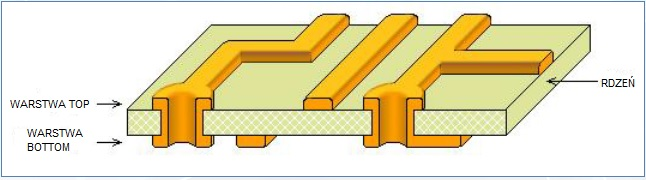
\includegraphics[width=\textwidth]{figures/Bez-tytulu}
\caption{Przekrój płytki PCB. Źródło:~\cite{Romik_TSPCB_ObwodDrukowany}.}\label{rys:przekroj-pcb}
\end{figure}

\subsection{Elementy PCB}

\begin{description}
  \item[Warstwa przewodząca] (ang.~\emph{conductive layer}) --- elementy
    przewodzące płytki leżące na tej samej warstwie, np.~ścieżki, płaszczyzny
    lub pady~\cite[pkt 3.2.18]{ECSS_Q_ST_70_12C_Rev1}.
  \item[Footprint] --- reprezentacja elementu elektronicznego na płytce wraz
    z jego padami~\cite{KiCad_PCBEditor_BasicConcepts}.
  \item[Pad] (pole lutownicze, ang.~\emph{soldering pad}) --- element
    przewodzący przeznaczony do przylutowania komponentu do
    płytki~\cite[pkt 3.2.62]{ECSS_Q_ST_70_12C_Rev1}.
  \item[Sieć] (ang.~\emph{net}) --- określenie, w jaki sposób pady mają być ze
    sobą połączone~\cite{KiCad_PCBEditor_BasicConcepts}.
  \item[Ścieżka] (ang.~\emph{track}) --- element przewodzący prowadzący
    połączenie elektryczne między padami~\cite[pkt 3.2.66]{ECSS_Q_ST_70_12C_Rev1}.
  \item[Przelotka] (ang.~\emph{via}) --- metalizowany otwór służący wyłącznie
    do łączenia warstw~\cite[pkt 3.2.67]{ECSS_Q_ST_70_12C_Rev1}.
  \item[Wypełniony obszar miedzi] (ang.~\emph{filled zone}) --- obszar miedzi
    tworzący, obok ścieżek i przelotek, połączenia między padami danej
    sieci~\cite{KiCad_PCBEditor_BasicConcepts}.
\end{description}

\section{Problem placementu}
\label{sec:problem-placementu}

% TODO: definicja problemu rozmieszczania elementów (dane wejściowe, wynik,
% ograniczenia, kryteria oceny -- analogicznie do sekcji o routingu).

\section{Problem routingu}

w problemie routingu, sieci są danymi wejściowymi a na wyjściu oczekuje się modelu fizycznego płytki. Jednak w praktyce
rozmieszczenie elementów na płytce jest z góry narzucone a zatem również można traktować je jako daną wejściową - co spłyca
problem routingu do samego prowadzenia ścieżek i rozmieszczania przelotek.

\begin{description}
  \item[Dane wejściowe] --- obrys płytki, liczba warstw, rozmieszczone
    footprinty, sieci oraz reguły projektowe.
  \item[Wynik] --- ścieżki i przelotki łączące pady każdej sieci.
  \item[Ograniczenia] --- brak zwarć między różnymi sieciami, zachowanie
    minimalnych odstępów i szerokości ścieżek.
  \item[Kryteria oceny] --- odsetek połączonych sieci, łączna długość ścieżek,
    liczba przelotek.
\end{description}

\section{Reguły projektowe}

Programy do projektowania płytek takie jak EasyEDA lub KiCad posiadają wbudowane narzędzie do weryfikacji,
czy określone wymagania dotyczące płytki zostały spełnione oraz czy wszystkie pady zostały połączone zgodnie z
netlistami. Narzędzie to nosi nazwę DRC (ang. Design Rule Checker). W przypadku KiCada narzędzie automatycznie
zapobiega łamaniu niektórych reguł podczas trasowania ścieżek. Nadal jednak istnieje wiele regół których w ten
sposób nie da się wykluczyć, gotowy schemat oraz przygotowaną płytkę należy zatem walidować.~\cite{KiCad_PCBEditor_DRC}:

\begin{description}
  \item[Minimalny odstęp izolacyjny] (ang.~\emph{clearance}) --- najmniejsza
    dopuszczalna odległość między elementami miedzi należącymi do różnych sieci.
  \item[Szerokość ścieżki] (ang.~\emph{track width}) --- minimalna, zalecana
    i~maksymalna szerokość ścieżki. Wraz z~odstępem izolacyjnym decyduje, ile
    ścieżek można poprowadzić między sąsiednimi padami.
  \item[Wymiary przelotki] --- średnica przelotki, średnica otworu oraz
    szerokość pierścienia miedzi wokół otworu (ang.~\emph{annular width}).
    Przelotka zajmuje miejsce na każdej warstwie, przez którą przechodzi.
  \item[Odstęp od krawędzi płytki] (ang.~\emph{edge clearance}) --- minimalna
    odległość miedzi od obrysu płytki, wynikająca z~tolerancji frezowania.
  \item[Odstęp obrysów elementów] (ang.~\emph{courtyard clearance}) ---
    minimalna odległość między obrysami zajmowanymi przez footprinty; ich
    nachodzenie na siebie jest błędem.
  \item[Obszary zabronione] (ang.~\emph{keepout}) --- obszary, w~których nie
    wolno umieszczać wskazanych obiektów, np.~ścieżek, przelotek lub footprintów.
  \item[Ograniczenia integralności sygnału] --- dopuszczalna długość połączenia
    (ang.~\emph{length}), różnica długości połączeń (ang.~\emph{skew}) oraz
    odstęp między ścieżkami pary różnicowej (ang.~\emph{differential pair gap}).
\end{description}

Za poprawne rozwiązanie problemu routingu można uznać takie, w~którym DRC nie
wykazuje zwarć między sieciami (\emph{Items shorting two nets}), naruszeń
odstępów (\emph{Clearance violation}) ani niepołączonych elementów sieci
(\emph{Missing connection between items})~\cite{KiCad_PCBEditor_DRC}.

Rozwiązania oparte na sztucznej inteligencji uwzględniają reguły projektowe
w~uproszczonej postaci. Zestawienie dla dwóch rozwiązań z~otwartym kodem
przedstawiono w~tabeli~\ref{tab:reguly-ai}.

\begin{table}[ht]
\fcmtcaption{Uwzględnienie reguł projektowych w~rozwiązaniach Unet-Astar
i~RL\_PCB. Źródło: opracowanie własne na podstawie kodu
źródłowego~\cite{Firesuiry_UnetAstar_GitHub,Vassallo_RLPCB_GitHub}.}\label{tab:reguly-ai}
\centering\footnotesize%
\begin{tabular}{p{0.22\textwidth} p{0.34\textwidth} p{0.34\textwidth}}
\toprule
Reguła & Unet-Astar (trasowanie) & RL\_PCB (rozmieszczanie) \\
\midrule
Odstęp izolacyjny & jedna wartość dla całej płytki, zaokrąglana w~górę do
  siatki & nie dotyczy \\
  \midrule
Szerokość ścieżki & jedna wartość dla całej płytki & nie dotyczy \\
\midrule
Klasy sieci & nieobsługiwane & nie dotyczy \\
\midrule
Wymiary przelotki & jeden rozmiar (najmniejszy z~pliku wejściowego) & nie
  dotyczy \\
  \midrule
Odstęp obrysów elementów & nie dotyczy (rozmieszczenie jest daną wejściową)
  & ograniczenie miękkie: kara w~funkcji nagrody; w~ocenie dopuszczano do
  20\% nakładania \\
  \midrule
Obrys elementu & nie dotyczy & prostokąt o~wymiarach elementu \\
\midrule
Orientacja elementu & nie dotyczy & obroty o~wielokrotność $90^\circ$ \\
\midrule
Trasowanie w~ocenie & --- & zewnętrzny program, z~pominięciem sieci zasilania \\
\bottomrule
\end{tabular}
\end{table}

% TODO ogólny opis algorytmów a nie zastosowanie ich w programach

\section{Algorytm A*}
A* jest heurystycznym algorytmem służącym do znajdowanias najkrótszej ścieżki w grafie.
Jest to algorytm zupełny i optymalny, a zatem zawsze da się znaleźć przy jego pomocy
najlepsze rozwiązanie. Metoda gwarantuje, że każdy punkt zostanie odwiedzony dzięki zorganizowanemu
modelowi pamięciowemu.

Działanie oparte jest na minimalizacji funkcji celu $f(x)$, zdefiniowanej jako suma funkcjo kosztu
$g(x)$ oraz funkcji heurystycznej $h(x)$:
\begin{equation}
  f(x) = g(x) + h(x)
  \label{eq:astar-f}
\end{equation}

W każdym krokui A* przedłuża już utworzoną ścieżkę o kolejny wierzchołek grafu wybierając taki,
w którym wartość funkcji $f$ będzie najmniejsza.

Funkcja $g(x)$ określa rzeczywisty koszt dojścia do punktu $x$ (suma wag krawędzi należących do ścieżki
oraz wagi krawędzi łączącej aktualny węzeł z $x$).

funkcja $h(x)$ funkcja heurystyczna. Oszacowuje w sposób optymistyczny koszt dotarcia od punktu $x$
do wierzchołka docelowego.

warunki prawidłowości funkcji heurystycznej:

warunek dopuszczalności
\begin{equation}
  g(x) + h(x) \le g(x_t),
  \label{eq:astar-dopuszczalnosc}
\end{equation}
gdzie $x_t$ oznacza punkt końcowy.

warunek monotoniczności
\begin{equation}
  g(x_j) + h(x_j) \ge g(x_i) + h(x_i),
  \label{eq:astar-monotonicznosc}
\end{equation}
gdzie $j > i$.

\subsection{Adaptacja algorytmu A* w~metodzie Unet-Astar}
\label{sec:astar-unet}

Algorytm trasowania w~metodzie Unet-Astar opiera się na algorytmie A*
zaproponowanym przez T.-C.~Lina i~in.\ do ujednoliconego trasowania płytek
PCB~\cite{Lin2021UnifiedPCB,Yin2023UnetAstar}. Płytkę przedstawia się jako
trójwymiarową siatkę, w~której węzeł odpowiada oczku siatki na danej
warstwie miedzi. Ścieżka jest drogą w~tym grafie między węzłami
odpowiadającymi dwóm padom, a~przejście między warstwami odpowiada
przelotce.

W~odróżnieniu od algorytmu bazowego Unet-Astar stosuje zmodyfikowaną funkcję
oceny węzła~\cite{Yin2023UnetAstar}:
\begin{equation}
  f(c) = g(s, c) + h(c, t) - P_{\mathrm{lin}} \cdot r(c),
  \label{eq:unet-astar-koszt}
\end{equation}
gdzie $g(s,c)$ oznacza koszt dojścia od punktu początkowego $s$ do bieżącego
węzła $c$, a~$h(c,t)$ oszacowanie kosztu dojścia od węzła $c$ do punktu
docelowego $t$. Koszt obejmuje długość ścieżki, karę za załamania
oraz karę za naruszenie reguł projektowych. Wartość $r(c) \in [0,1]$ to
wartość obszaru rekomendowanego w~węźle $c$, przewidziana przez sieć
neuronową przed rozpoczęciem trasowania połączenia. Hiperparametr
$P_{\mathrm{lin}}$ (ang.~\emph{liner-power}) określa kompromis między
podążaniem za obszarem rekomendowanym a~kosztem trasowania. Im większa jego
wartość, tym silniej algorytm preferuje węzły wskazane przez sieć i~tym
mniej węzłów spoza obszaru rekomendowanego rozwija. Odjęcie składnika
zależnego od $r(c)$ sprawia, że heurystyka przestaje być dopuszczalna
w~sensie warunku~(\ref{eq:astar-dopuszczalnosc}). Algorytm nie gwarantuje
więc już ścieżki o~najmniejszym koszcie, ale w~zamian przeszukuje znacznie
mniejszą część siatki.

Wiele krótkich połączeń na płytce jest na tyle prostych, że obszar
rekomendowany niewiele przyspiesza ich poprowadzenie. Dlatego wprowadzono
drugi hiperparametr, $p_{\mathrm{skip}}$ (ang.~\emph{skip-percent}).
Połączenia szereguje się według długości. Następnie najkrótsze połączenia
stanowiące \emph{skip-percent} wszystkich połączeń prowadzi się
klasycznym algorytmem A*, bez użycia sieci~\cite{Yin2023UnetAstar}.
Analogicznie połączenia te pomija się przy tworzeniu próbek
uczących.

Trasowanie całej płytki przebiega w~następujących krokach~\cite{Yin2023UnetAstar}:
\begin{enumerate}
  \item Sieci wielopinowe dzieli się na połączenia dwupinowe za pomocą
    algorytmu drzewa Steinera.
  \item Połączenia dwupinowe szereguje się według długości odcinka łączącego
    ich końce, od najkrótszego do najdłuższego.
  \item Połączenia prowadzi się kolejno, zgodnie z~ustaloną kolejnością.
\end{enumerate}
Połączenia prowadzone są sekwencyjnie, więc każda poprowadzona ścieżka staje
się przeszkodą dla kolejnych. Na dużych i~gęstych płytkach algorytm A*
musi wtedy rozwinąć bardzo wiele węzłów, zanim znajdzie drogę omijającą
wcześniej poprowadzone ścieżki. Ograniczenie przeszukiwanego obszaru za
pomocą predykcji sieci neuronowej jest odpowiedzią właśnie na ten
problem.

\section{Algorytm Lee}
\label{sec:lee}

Algorytm Lee, zaproponowany przez C.~Y.~Lee w~1961~roku, służy do
wyznaczania połączenia między dwoma punktami na siatce z~przeszkodami.
Został opracowany z~myślą o~prowadzeniu połączeń w~układach
elektronicznych i~jest jednym z~pierwszych algorytmów trasowania płytek
drukowanych~\cite{Lee1961}. Płytkę przedstawia się jako siatkę oczek,
z~których każde jest wolne albo zajęte przez przeszkodę. Algorytm działa
w~dwóch fazach:
\begin{enumerate}
  \item \emph{Propagacja fali} --- oczko początkowe otrzymuje etykietę~0.
    Następnie wszystkie wolne, nieoznaczone sąsiednie oczka oczek
    z~etykietą $k$ otrzymują etykietę $k+1$. Fala rozchodzi się w~ten sposób
    równomiernie we wszystkich kierunkach, aż dotrze do oczka docelowego
    albo nie będzie już oczek do oznaczenia.
  \item \emph{Odtworzenie ścieżki} --- począwszy od oczka docelowego
    przechodzi się do dowolnego sąsiada o~etykiecie mniejszej o~1, aż do
    oczka początkowego. Uzyskany ciąg oczek jest najkrótszą ścieżką.
\end{enumerate}

Algorytm zawsze znajduje najkrótszą ścieżkę, jeżeli taka istnieje, ale
w~najgorszym przypadku oznacza wszystkie oczka siatki. Czas działania
i~zapotrzebowanie na pamięć rosną więc proporcjonalnie do powierzchni płytki:
dla siatki o~wymiarach $M \times N$ oczek wynoszą $O(MN)$~\cite{Zhou_EECS357_Lee}.
W~odróżnieniu od algorytmu A* propagacja nie jest kierowana heurystyką
w~stronę celu, dlatego algorytm odwiedza znacznie więcej oczek.

W~metodzie Unet-Astar dwukierunkowy wariant algorytmu Lee służy do
przygotowania danych uczących~\cite{Yin2023UnetAstar}. Fale propagowane są
jednocześnie z~punktu początkowego $s$ i~końcowego $t$, dzięki czemu dla
każdego oczka $n$ znane są odległości $d_s(n)$ i~$d_t(n)$ od obu końców
połączenia. Obszar rekomendowany tworzą oczka, przez które przechodzi
ścieżka niewiele dłuższa od najkrótszej:
\begin{equation}
  R = \{\, n : d_s(n) + d_t(n) \le L^* + 0{,}1 \cdot d(s, t) \,\},
  \label{eq:lee-obszar}
\end{equation}
gdzie $L^*$ oznacza długość najkrótszej ścieżki, a~$d(s,t)$ odległość
euklidesową między końcami połączenia~\cite{Yin2023UnetAstar}. Tak
wyznaczone obszary stanowią etykiety, na których uczona jest sieć
neuronowa. Podczas trasowania algorytm Lee nie jest już wykonywany ---
obszar rekomendowany przewiduje wytrenowana sieć.

\section{Konwolucyjne sieci neuronowe}

Konwolucyjne sieci neuronowe (ang.~\emph{convolutional neural networks}, CNN)
są zbudowane, podobnie jak klasyczne sieci neuronowe, z~neuronów, które
uczą się przez optymalizację swoich wag. Każdy neuron otrzymuje sygnały
wejściowe i~wykonuje na nich operację, np.~iloczyn skalarny, po którym
następuje nieliniowa funkcja aktywacji. Sieci te są stosowane przede
wszystkim do rozpoznawania wzorców w~obrazach, a~ich architektura
uwzględnia cechy tego rodzaju danych~\cite{OShea2015CNN}.

W~klasycznej sieci każdy neuron pierwszej warstwy ukrytej jest połączony
ze wszystkimi wartościami wejściowymi. Dla kolorowego obrazu o~wymiarach
$64 \times 64$ oznacza to $64 \cdot 64 \cdot 3 = 12\,288$ wag w~jednym
neuronie. Tak duża liczba parametrów wymaga dużej mocy obliczeniowej
i~zwiększa ryzyko przeuczenia (ang.~\emph{overfitting}), czyli utraty
zdolności uogólniania na dane spoza zbioru uczącego~\cite{OShea2015CNN}.

W~sieci konwolucyjnej neurony są uporządkowane w~trzech wymiarach:
wysokości, szerokości i~głębokości. Głębokość oznacza tu trzeci wymiar
danych, np.~liczbę kanałów obrazu, a~nie liczbę warstw sieci. Każdy neuron
jest połączony tylko z~niewielkim obszarem poprzedniej warstwy. Sieć
składa się z~trzech rodzajów warstw: konwolucyjnych, łączących
(ang.~\emph{pooling}) i~w~pełni połączonych~\cite{OShea2015CNN}.


\section{U-net}
- Rodzaj sieci konwolucyjnej, w skrócie: konwolucja, pooling, segmentacja obrazu 
(klasyfikacja każdego pixela).
- Część kodująca zmiejsza obraz i zbiera kontekst, a część dekodująca odtwarza rozdzielczość.
- Połączenia pomijające (skip connections) przekazują szczegóły przestrzenne z kodera do dekodera.

\section{Deeper U-Net i Unet-Astar}
- Pomysł z Artykułu: sieć wskazuje obszary rekomendowane, a głębsza struktura daje więcej informacji kontekstowej.
- Architektura w kodzie: wejście $256 \times 256$ z 3 kanałami, 8 redukcji rozdzielczości aż do $1 \times 1$, warstwa w pełni połączona
w środku i 2 klasy na wyjściu. Klasyczny U-Net ma 4 redukcje.
- Połączenie z A*: sieć nie zastępuje A*, tylko zmienia kolejność odwiedzania węzłów

\begin{equation}
  f'(n) = \bigl(f(n) - a \cdot s(n)\bigr) \cdot \bigl(1 - b \cdot s(n)\bigr),
  \label{eq:unet-astar-f}
\end{equation}
gdzie $s(n)$ to wynik sieci dla węzła, a domyślnie $a = b = 3$.
Dla $b = 0$ wzór sprowadza się do funkcji~(\ref{eq:unet-astar-koszt})
z~artykułu, przy $a = P_{\mathrm{lin}}$.

\section{Reinforcement Learning}

%TODO opis ogólny RL oraz adaptacja architektury sieci w RL PCB
\chapter{Rozwinięcie}
\label{ch:rozwiniecie}

W~rozdziale opisano przedmiot i~metodykę badań. Przedstawiono cel badań,
przebieg eksperymentu, sposób przygotowania danych uczących i~testowych,
porównywane warianty trasowania oraz miary, według których je oceniano.

% TODO: część dotycząca RL_PCB (rozmieszczanie elementów).

\section{Cel badań}
\label{sec:cel-badan}

Celem badań jest ocena, czy rozwiązanie Unet-Astar~\cite{Yin2023UnetAstar}
wytrenowane wyłącznie na syntetycznych, losowo generowanych płytkach może
skutecznie wspierać trasowanie rzeczywistych projektów PCB. Sformułowano
następujące pytania badawcze:
\begin{enumerate}
  \item Czy predykcja sieci U-Net zmniejsza liczbę węzłów rozwijanych przez
    algorytm A* na płytkach rzeczywistych, a~więc czy sieć uogólnia się poza
    rozkład danych uczących?
  \item Jak jakość trasowania uzyskanego algorytmem Unet-Astar (odsetek
    połączonych sieci, długość ścieżek, liczba przelotek, liczba naruszeń reguł
    projektowych) wypada na tle autoroutera wbudowanego w~EasyEDA?
  \item Czy różnice w~geometrii ścieżek przekładają się na właściwości istotne
    z~punktu widzenia kompatybilności elektromagnetycznej?
\end{enumerate}

\section{Przebieg badań}
\label{sec:przebieg-badan}

Algorytm Unet-Astar nie wyznacza ścieżek samodzielnie --- sieć neuronowa
jedynie zmienia kolejność rozwijania węzłów przez A*
(wzór~\ref{eq:unet-astar-f}). Wpływ sieci na jakość trasowania jest więc
pośredni, a~jej główną zaletą ma być skrócenie wyszukiwania. Z~tego powodu
porównanie wyłącznie z~autorouterem EasyEDA nie pozwoliłoby rozdzielić wpływu
sieci od wpływu samego algorytmu A*. W~badaniach porównano zatem trzy warianty
trasowania:
\begin{description}
  \item[EasyEDA] --- wbudowany autorouter EasyEDA (wariant odniesienia);
  \item[A*] --- algorytm wielowarstwowego A* z~repozytorium Unet-Astar
    uruchomiony bez sieci neuronowej;
  \item[Unet-A*] --- ten sam algorytm wspomagany predykcją sieci U-Net.
\end{description}

Badania przebiegały w~następujących krokach:
\begin{enumerate}
  \item Wygenerowanie zbioru uczącego z~losowych płytek
    (sekcja~\ref{sec:zbior-uczacy}).
  \item Trening sieci U-Net (sekcja~\ref{sec:trening}).
  \item Przygotowanie płytek testowych w~EasyEDA: projektów własnych oraz
    zaimportowanych projektów gotowych (sekcja~\ref{sec:zbior-testowy}).
  \item Trasowanie każdej płytki testowej autorouterem EasyEDA i~eksport
    pliku autoroutera w~formacie \emph{Specctra DSN}.
  \item Trasowanie tej samej płytki na podstawie pliku DSN w~wariantach A*
    i~Unet-A*.
  \item Import wyniku (plik \emph{Specctra SES}) z~powrotem do EasyEDA,
    weryfikacja DRC i~odczyt statystyk projektu.
  \item Zestawienie miar (sekcja~\ref{sec:miary}) dla wszystkich płytek
    testowych i~wariantów.
\end{enumerate}

Wszystkie warianty otrzymują identyczne dane wejściowe: obrys płytki, rozmieszczenie
elementów, sieci oraz reguły projektowe zapisane w~tym samym pliku DSN.

\section{Środowisko badawcze}
\label{sec:srodowisko}

\begin{table}[ht]
\fcmtcaption{Środowisko badawcze. Źródło: opracowanie własne.}\label{tab:srodowisko}
\centering\footnotesize%
\begin{tabular}{p{0.3\textwidth} p{0.6\textwidth}}
\toprule
Element & Wersja / parametry \\
\midrule
System operacyjny & Windows 11 Home \\
\midrule
Procesor & Intel Core i5-8400, 2,8~GHz, 6~rdzeni / 6~wątków \\
\midrule
Pamięć RAM & 24~GB, 2133~MT/s \\
\midrule
Karta graficzna & NVIDIA GeForce GTX 1060, 3~GB \\
\midrule
Python & 3.8.10 \\
\midrule
PyTorch & 2.4.1 (CUDA 12.1) \\
\midrule
EasyEDA & Standard, wersja 6.5.61 \\
\midrule
Unet-Astar & repozytorium~\cite{Firesuiry_UnetAstar_GitHub} wraz
  z~modyfikacjami opisanymi w~sekcji~\ref{sec:modyfikacje} \\
\bottomrule
\end{tabular}
\end{table}

\section{Format danych i~współpraca z~EasyEDA}
\label{sec:format-danych}

Wymiana danych z~EasyEDA odbywa się za pośrednictwem plików autoroutera
w~formacie \emph{Specctra}. Plik DSN zawiera obrys płytki, definicje warstw,
reguły projektowe (odstęp izolacyjny, szerokość ścieżki, przelotki), kształty
padów (\emph{padstack}), położenia pinów oraz listę sieci. EasyEDA zapisuje
płytkę jako jeden komponent, którego piny mają współrzędne bezwzględne.
Obroty elementów są uwzględnione bezpośrednio w~kształtach padów.
Współrzędne zapisane są w~jednostkach EasyEDA równych 10~mil.

Program Unet-Astar przelicza współrzędne na mile i~na potrzeby trasowania
przenosi je na siatkę o~boku 8~mil (ok.~0{,}2~mm). Reguły projektowe są przy
tym zaokrąglane w~górę do całkowitej liczby oczek siatki.

Oryginalny program Unet-Astar nie zapisuje wyniku w~formacie, który można
wczytać z~powrotem do EasyEDA. Wymiana danych przebiega więc w~dwóch
kierunkach: z~EasyEDA eksportowany jest plik DSN, będący danymi wejściowymi
programu Unet-Astar, a~wynik trasowania wraca do EasyEDA jako plik sesji
\emph{Specctra SES} importowany do projektu.
Plik SES generowany jest przez eksporter przygotowany na potrzeby badań.
Eksporter odwzorowuje kolejne punkty ścieżki z~siatki
z~powrotem na współrzędne płytki, zmianę warstwy zapisuje jako przelotkę,
a~ścieżki podsieci powstałych z~podziału sieci wielopinowych łączy pod
wspólną nazwą sieci z~pliku DSN. Szerokość ścieżki i~średnicę przelotki
przyjmuje się z~reguł zapisanych w~pliku DSN, bez zaokrąglenia do siatki.
Ponieważ siatka o~boku 8~mil nie pokrywa się ze środkami padów, końce
ścieżek dociągane są krótkim odcinkiem do środka padu. Odcinek ten
może naruszać reguły odstępów, dlatego zaimportowana płytka jest
sprawdzana narzędziem DRC programu EasyEDA.

\section{Zbiór uczący}
\label{sec:zbior-uczacy}

Sieć trenowano wyłącznie na płytkach syntetycznych, generowanych losowo zgodnie
z~procedurą z~repozytorium Unet-Astar. Parametry generatora zestawiono
w~tabeli~\ref{tab:generator}.

\begin{table}[ht]
\fcmtcaption{Parametry generatora losowych płytek. Źródło: opracowanie własne
na podstawie kodu źródłowego~\cite{Firesuiry_UnetAstar_GitHub}.}\label{tab:generator}
\centering\footnotesize%
\begin{tabular}{p{0.45\textwidth} p{0.45\textwidth}}
\toprule
Parametr & Wartość \\
\midrule
Liczba płytek & 1250 \\
\midrule
Wymiary płytki & losowo 1000--2000~mil (25{,}4--50{,}8~mm) w~każdej osi \\
\midrule
Liczba warstw & 2 \\
\midrule
Gęstość pinów & 0{,}15 pinu na pole $100 \times 100$~mil \\
\midrule
Gęstość przeszkód & 0{,}1 przeszkody na pole $300 \times 300$~mil \\
\midrule
Kształty padów & koło o~średnicy 80~mil lub prostokąt $56 \times 48$~mil \\
\midrule
Przeszkody & koło o~średnicy 240~mil, bez przypisanej sieci \\
\midrule
Minimalne odległości & pin--pin 100~mil, pin--przeszkoda 300~mil,
  przeszkoda--przeszkoda 500~mil \\
  \midrule
Sieci & wyłącznie dwupinowe, piny przydzielane losowo \\
\midrule
Siatka trasowania & 8~mil \\
\bottomrule
\end{tabular}
\end{table}

Górną granicę wymiarów płytki dobrano tak, aby płytka mieściła się w~wejściu
sieci o~rozmiarze $256 \times 256$ oczek siatki (2048~mil). W~oryginalnym
repozytorium generowano płytki do 5000~mil, jednak próbki większe od wejścia
sieci są odrzucane przez moduł wczytujący dane.

Każda wygenerowana płytka jest najpierw w~całości trasowana algorytmem A*.
Sieci są prowadzone kolejno, od najkrótszej. Następnie dla każdego połączenia
(z~pominięciem 30\% najkrótszych) tworzona jest próbka ucząca:
\begin{description}
  \item[Wejście] --- obraz o~trzech kanałach. Kanał pierwszy zawiera punkt
    początkowy i~końcowy połączenia rozmyte filtrem Gaussa o~odchyleniu
    standardowym równym 30\% odległości między nimi. Kanały drugi i~trzeci
    zawierają mapy przeszkód na obu warstwach: pady innych sieci oraz
    pozostałe, już poprowadzone ścieżki.
  \item[Etykieta] --- dwukanałowa maska obszaru rekomendowanego,
    wyznaczona dwukierunkowym algorytmem Lee (sekcja~\ref{sec:lee}).
\end{description}

Algorytm Lee służy wyłącznie do przygotowania etykiet. Wyznacza obszar
rekomendowany dokładnie, ale przeszukuje przy tym całą dostępną część
płytki, więc nie przyspieszyłby trasowania. Sieć uczy się odtwarzać jego
wynik: kosztowne obliczenia wykonywane są jednokrotnie, podczas generowania
zbioru uczącego, a~w~trakcie trasowania zastępuje je pojedyncza predykcja
sieci. Jakość obszarów wyznaczonych przez algorytm Lee stanowi zatem górną
granicę tego, czego sieć może się nauczyć.

Implementacja w~repozytorium różni się od opisu w~artykule
(wzór~\ref{eq:lee-obszar}). Do obszaru rekomendowanego należą oczka
spełniające warunek $d_s(n) + d_t(n) \le L^* + 0{,}1\,d_M(s,t) + 1$, gdzie
$d_M$ oznacza odległość w~metryce miejskiej zamiast euklidesowej, a~stały
składnik $+1$ poszerza obszar o~jedno oczko zapasu. W~badaniach
wykorzystano etykiety wyznaczone zgodnie z~implementacją.

Uzyskano 13\,830 próbek. Zbiór podzielono losowo w~proporcji
90:10 na część uczącą i~walidacyjną.

\section{Model i~trening}
\label{sec:trening}

Repozytorium zawiera trzy architektury: klasyczny U-Net (31~mln parametrów),
U-Net++ (47~mln) oraz głęboką sieć \emph{ResNetUNet} zaproponowaną przez
autorów rozwiązania (170~mln parametrów, 8~poziomów redukcji rozdzielczości).
Próba treningu modelu \emph{ResNetUNet} na dostępnej karcie graficznej
z~3~GB pamięci wykazała, że już przy dwóch próbkach w~paczce zapotrzebowanie
na pamięć przekracza jej pojemność. Trening trwał wówczas ponad 4~s na
paczkę. Z~tego powodu w~badaniach wykorzystano klasyczny U-Net, który przy
czterech próbkach w~paczce zajmuje ok.~2~GB pamięci.
% TODO: Google Colab -- dopisać.

\begin{table}[ht]
\fcmtcaption{Parametry treningu. Źródło: opracowanie własne.}\label{tab:trening}
\centering\footnotesize%
\begin{tabular}{p{0.45\textwidth} p{0.45\textwidth}}
\toprule
Parametr & Wartość \\
\midrule
Architektura & U-Net, wejście $3 \times 256 \times 256$, wyjście
  $2 \times 256 \times 256$ \\
  \midrule
Funkcja straty & $0{,}5 \cdot \mathrm{BCE} + 0{,}5 \cdot \mathrm{Dice}$ \\
\midrule
Optymalizator & Adam, współczynnik uczenia $10^{-4}$ \\
\midrule
Harmonogram & mnożenie współczynnika uczenia przez 0{,}75 po każdej epoce \\
\midrule
Liczba epok & 15 \\
\midrule
Rozmiar paczki & 4 \\
\midrule
Wybór modelu & najmniejsza strata na zbiorze walidacyjnym \\
\bottomrule
\end{tabular}
\end{table}

W~trakcie trasowania sieć wywoływana jest dla każdego połączenia
z~wyjątkiem 30\% najkrótszych. Dla płytek większych od wejścia sieci
z~mapy przeszkód wycinany jest fragment $256 \times 256$ oczek
wyśrodkowany między punktami połączenia. Połączenia, których rozpiętość
w~którejkolwiek osi przekracza 256 oczek, prowadzone są bez udziału sieci.
Wynik sieci $s(n)$ modyfikuje funkcję oceny węzła zgodnie ze
wzorem~\ref{eq:unet-astar-f}, z~parametrami $a = 800$ i~$b = 0$,
przyjętymi za eksperymentami autorów.

\section{Zbiór testowy}
\label{sec:zbior-testowy}

Zbiór testowy obejmuje wyłącznie płytki rzeczywiste, niewykorzystane
w~treningu:
\begin{itemize}
  \item płytki zaprojektowane samodzielnie w~EasyEDA,
  \item gotowe projekty udostępnione publicznie w~serwisie EasyEDA ---
    projekt przykładowy \emph{Project-Sample} z~sekcji
    \emph{Modules}~\cite{EasyEDA_ProjectSample}.
\end{itemize}

Z~zaimportowanych projektów przed trasowaniem usuwane są ścieżki
i~przelotki poprowadzone przez ich autorów, tak aby wszystkie warianty
trasowały płytkę od początku. Ścieżki zapisane w~pliku DSN (sekcja
\emph{wiring}) są przez program Unet-Astar pomijane.
Ze względu na ograniczenia rozwiązania płytki testowe muszą spełniać
następujące warunki:
\begin{itemize}
  \item dwie warstwy miedzi --- sieć przyjmuje mapy przeszkód dokładnie
    dwóch warstw;
  \item obrys prostokątny --- program uwzględnia wyłącznie prostokąt
    opisany na obrysie płytki;
  \item brak obszarów zabronionych i~stref miedzi --- nie są one
    odczytywane z~pliku DSN.
\end{itemize}
Płytki większe niż $2048 \times 2048$~mil mogą być trasowane, ale miary
jakości predykcji (sekcja~\ref{sec:miary}) wyznaczane są wyłącznie dla
płytek mieszczących się w~wejściu sieci.

Rozkład danych testowych istotnie różni się od rozkładu danych uczących.
Płytki rzeczywiste zawierają sieci wielopinowe, które program dzieli na
połączenia dwupinowe. Mają też gęsto rozmieszczone pady elementów SMD
o~różnych kształtach i~nierównomierne zagęszczenie połączeń. Badanie
ma zatem charakter oceny zdolności uogólniania modelu.

\section{Miary oceny}
\label{sec:miary}

Miary zestawiono w~tabeli~\ref{tab:miary}. Miary jakości trasowania
odczytywane są w~EasyEDA po zaimportowaniu wyniku, dzięki czemu wszystkie
warianty oceniane są tym samym narzędziem. Miary wydajności wyszukiwania
dotyczą wyłącznie wariantów A* i~Unet-A*.

\begin{table}[ht]
\fcmtcaption{Miary oceny. Źródło: opracowanie własne.}\label{tab:miary}
\centering\footnotesize%
\begin{tabular}{p{0.28\textwidth} p{0.42\textwidth} p{0.2\textwidth}}
\toprule
Miara & Opis & Warianty \\
\midrule
\multicolumn{3}{l}{\emph{Jakość trasowania}} \\
\midrule
Odsetek połączeń & udział poprowadzonych połączeń w~liczbie wszystkich
  połączeń & wszystkie \\
  \midrule
Długość ścieżek & łączna długość ścieżek na obu warstwach & wszystkie \\
\midrule
Liczba przelotek & --- & wszystkie \\
\midrule
Naruszenia DRC & liczba błędów zgłoszonych przez DRC EasyEDA, w~podziale
  na typy & wszystkie \\
  \midrule
Czas trasowania & czas od wczytania płytki do zakończenia trasowania
  & wszystkie \\
\midrule
\multicolumn{3}{l}{\emph{Wydajność wyszukiwania}} \\
\midrule
Rozwinięte węzły & liczba węzłów rozwiniętych przez A*; miara niezależna
  od implementacji i~sprzętu & A*, Unet-A* \\
  \midrule
Redukcja węzłów & $1 - N_{\mathrm{U}} / N_{\mathrm{A}}$, gdzie
  $N_{\mathrm{U}}$ i~$N_{\mathrm{A}}$ to liczby węzłów rozwiniętych przez
  Unet-A* i~A*; liczona dla połączeń, w~których użyto sieci & Unet-A* \\
\midrule
\multicolumn{3}{l}{\emph{Jakość predykcji}} \\
\midrule
Dice, IoU & zgodność maski przewidzianej przez sieć (próg 0{,}5)
  z~etykietą wyznaczoną algorytmem Lee & Unet-A* \\
\bottomrule
\end{tabular}
\end{table}

Wyniki dla każdej płytki testowej zapisywane są w~osobnym pliku, a~następnie
agregowane dla całego zbioru testowego.

\section{Ocena kompatybilności elektromagnetycznej}
\label{sec:emc}

% EMI jeśli się uda
Środowisko EasyEDA nie udostępnia symulacji pola elektromagnetycznego płytki.
Bezpośrednia ocena emisji zakłóceń wymagałaby zewnętrznego symulatora pola
albo pomiarów fizycznych wykonanych płytek. Z~tego powodu w~badaniach
zastosowano miary pośrednie, wyznaczane z~geometrii ścieżek. Są one zgodne
z~powszechnie stosowanymi zaleceniami projektowania pod kątem EMC:
\begin{itemize}
  \item łączna długość ścieżek --- dłuższe ścieżki skuteczniej promieniują
    i~odbierają zakłócenia;
  \item liczba przelotek --- każda przelotka stanowi nieciągłość impedancji;
  \item długość równoległego prowadzenia ścieżek różnych sieci w~odległości
    mniejszej niż zadany próg --- miara podatności na przesłuch;
  \item pole pętli tworzonej przez ścieżkę sygnałową i~ścieżkę powrotną
    masy --- miara emisji promieniowanej.
\end{itemize}
% openEMS; uzupełnić bibliografię o źródło zaleceń EMC.

\section{Modyfikacje kodu źródłowego}
\label{sec:modyfikacje}

Kod repozytorium Unet-Astar w~udostępnionej postaci nie umożliwiał
przeprowadzenia badań bez zmian. Wprowadzono następujące modyfikacje:
\begin{itemize}
  \item poprawiono wyznaczanie punktu początkowego i~końcowego próbki uczącej
    dla płytek wczytanych z~pliku DSN --- wykorzystywano współrzędne
    nieprzesunięte do początku układu, co dla płytek z~EasyEDA dawało
    ujemne indeksy;
  \item ujednolicono wartość zwracaną przez algorytm A* w~przypadku
    braku ścieżki --- wcześniej powodowała ona przerwanie przetwarzania
    całej płytki;
  \item poprawiono błąd indeksowania sieci w~module wizualizacji, który
    uniemożliwiał trasowanie płytek z~sieciami wielopinowymi;
  \item dodano zapis obiektu płytki wczytanej z~pliku DSN;
  \item dodano skrypty: generowania próbek z~losowych płytek i~z~plików DSN,
    treningu oraz testowania na płytkach z~EasyEDA;
  \item dodano zapis wyników trasowania do plików graficznych i~JSON;
  \item dodano eksport wyniku trasowania do pliku Specctra SES
    importowanego przez EasyEDA.
\end{itemize}

\section{Ograniczenia}
\label{sec:ograniczenia}

\begin{itemize}
  \item Trasowanie odbywa się na siatce 8~mil, a~reguły projektowe są
    zaokrąglane w~górę do jej wielokrotności. Skutkuje to większymi
    odstępami niż wymagane i~może uniemożliwić poprowadzenie ścieżek
    na gęstych płytkach.
  \item Program stosuje jedną szerokość ścieżki i~jeden odstęp dla całej
    płytki --- klasy sieci nie są obsługiwane (tabela~\ref{tab:reguly-ai}).
  \item Ze względu na pojemność pamięci karty graficznej nie wytrenowano
    modelu \emph{ResNetUNet} zaproponowanego przez autorów rozwiązania.
  \item Czasy działania zmierzone dla implementacji w~języku Python nie są
    porównywalne z~czasem działania autoroutera EasyEDA. Dlatego jako
    podstawową miarę wydajności przyjęto liczbę rozwiniętych węzłów.
\end{itemize}

\chapter{Badania}
\label{ch:badania}

W~rozdziale opisano przebieg eksperymentu przeprowadzonego zgodnie
z~metodyką przedstawioną w~rozdziale~\ref{ch:rozwiniecie}. Kolejne etapy,
wykorzystywane w~nich narzędzia oraz ich wyniki zestawiono
w~tabeli~\ref{tab:etapy}. Uzyskane wyniki omówiono
w~rozdziale~\ref{ch:wyniki}.

\begin{table}[ht]
\fcmtcaption{Etapy eksperymentu. Źródło: opracowanie własne.}\label{tab:etapy}
\centering\footnotesize%
\begin{tabular}{p{0.04\textwidth} p{0.33\textwidth} p{0.2\textwidth} p{0.3\textwidth}}
\toprule
Lp. & Etap & Narzędzie & Wynik \\
\midrule
1 & Generowanie zbioru uczącego i~trening sieci & Unet-Astar & wagi modelu U-Net \\
\midrule
2 & Utworzenie płytek testowych na podstawie schematów & EasyEDA & projekty PCB \\
\midrule
3 & Trasowanie płytek autorouterem & EasyEDA & wariant \emph{EasyEDA} \\
\midrule
4 & Eksport płytek do formatu Specctra & EasyEDA & pliki DSN \\
\midrule
5 & Trasowanie na podstawie plików DSN & Unet-Astar & ścieżki wariantów
  \emph{A*} i~\emph{Unet-A*}, statystyki wyszukiwania \\
  \midrule
6 & Eksport ścieżek & eksporter SES & pliki SES \\
\midrule
7 & Sklonowanie płytek i~naniesienie wyników & EasyEDA & płytki wariantów
  \emph{A*} i~\emph{Unet-A*} \\
  \midrule
8 & Odczyt parametrów płytek & EasyEDA & miary jakości trasowania \\
\midrule
9 & Zestawienie wyników & arkusz / skrypt & tabele porównawcze \\
\bottomrule
\end{tabular}
\end{table}

\section{Przygotowanie sieci neuronowej}
\label{sec:exp-trening}

Zbiór uczący wygenerowano zgodnie z~opisem w~sekcji~\ref{sec:zbior-uczacy}.
Utworzono 1250~losowych płytek dwuwarstwowych o~bokach od 1000 do
2000~mil. Generowanie prowadzono równolegle w~pięciu procesach.
Z~płytek uzyskano łącznie 13830~próbek (średnio ok.~11 na płytkę),
zajmujących na dysku 3,1~GB. Zbiór podzielono losowo w~proporcji 9:1 na
część uczącą i~walidacyjną.

Sieć U-Net trenowano z~parametrami podanymi w~tabeli~\ref{tab:trening}.
Do dalszych badań wybrano model o~najmniejszej stracie na zbiorze
walidacyjnym. Trening na karcie graficznej trwał łącznie 13~h 27~min
(15~epok, średnio ok.~54~min na epokę). Strata walidacyjna malała niemal
w~każdej epoce, z~0,155 po pierwszej do 0,098 po ostatniej. Najmniejszą
stratę walidacyjną (0,0978, w~tym BCE 0,0486 i~strata Dice 0,1471)
osiągnięto w~ostatniej, 15.~epoce. Oznacza to, że dłuższy trening mógłby
jeszcze nieznacznie poprawić model.
Przebieg funkcji straty przedstawiono w~rozdziale~\ref{ch:wyniki}.

\section{Przygotowanie płytek testowych}
\label{sec:exp-plytki}

Płytki testowe utworzono w~EasyEDA na podstawie dwóch rodzajów schematów:
\begin{itemize}
  \item schematów własnych,
  \item schematu publicznego projektu przykładowego \emph{Project-Sample},
    udostępnionego w~sekcji \emph{Modules} serwisu
    EasyEDA~\cite{EasyEDA_ProjectSample}.
\end{itemize}

Dla każdego schematu wygenerowano w~EasyEDA płytkę PCB, na której
umieszczono footprinty elementów wraz z~siecią połączeń. Następnie
wyznaczono prostokątny obrys płytki i~rozmieszczono elementy
ręcznie. Rozmieszczenie elementów nie było zmieniane w~dalszych etapach, 
dlatego wszystkie warianty trasowania otrzymują identyczne położenia padów. 
Płytki spełniają wymagania podane w~sekcji~\ref{sec:zbior-testowy}:
mają dwie warstwy miedzi, prostokątny obrys i~nie zawierają 
stref miedzi ani obszarów zabronionych.

Dla wszystkich płytek i~wszystkich sieci zastosowano ten sam zestaw reguł
projektowych (tabela~\ref{tab:reguly}). Reguły te zapisywane są w~pliku DSN
i~obowiązują wszystkie trzy warianty trasowania. W~programie Unet-Astar są
one zaokrąglane w~górę do całkowitej liczby oczek siatki
(sekcja~\ref{sec:format-danych}).

\begin{table}[ht]
\fcmtcaption{Reguły projektowe płytek testowych. Źródło: opracowanie własne.}\label{tab:reguly}
\centering\footnotesize%
\begin{tabular}{l r r}
\toprule
Reguła (wartość minimalna) & [mm] & [mil] \\
\midrule
Szerokość ścieżki & 0{,}254 & 10 \\
\midrule
Odstęp izolacyjny (\emph{clearance}) & 0{,}152 & 6 \\
\midrule
Średnica przelotki & 0{,}610 & 24 \\
\midrule
Średnica otworu przelotki & 0{,}305 & 12 \\
\bottomrule
\end{tabular}
\end{table}

Charakterystykę płytek testowych zestawiono w~tabeli~\ref{tab:plytki-testowe}.

\begin{table}[ht]
\fcmtcaption{Płytki testowe. Źródło: opracowanie własne.}\label{tab:plytki-testowe}
\centering\footnotesize%
\begin{tabular}{l l r r r r}
\toprule
Płytka & Pochodzenie & Wymiary [mm] & Elementy & Sieci & Połączenia \\
\midrule
Płytka z~diodą LED & własna & $51 \times 34$ & 4 & 4 & 4 \\
\midrule
Płytka przykładowa & publiczna & $37 \times 25$ & 8 & 6 & 16 \\
\bottomrule
\end{tabular}
\end{table}

Kolumna \emph{Połączenia} podaje liczbę połączeń dwupinowych, na które
program Unet-Astar dzieli sieci wielopinowe. Odpowiada ona liczbie
zadań wyszukiwania ścieżki wykonywanych przez algorytm A*. Na płytce
przykładowej jedna z~sześciu sieci ma tylko jeden pin, więc nie wymaga
poprowadzenia. Pozostałe pięć sieci, w~tym ośmiopinowa sieć zasilania
+24~V, daje łącznie 16~połączeń.

\section{Trasowanie autorouterem EasyEDA}
\label{sec:exp-autorouter}

Każdą płytkę testową poprowadzono autorouterem wbudowanym w~EasyEDA
(EasyEDA Standard 6.5.61, tabela~\ref{tab:srodowisko}). Reguły trasowania
autoroutera (\emph{Routing Rules}) odwołują się do reguł projektowych
(\emph{Design Rules}) zdefiniowanych dla projektu. Autorouter korzystał
więc z~tych samych wartości szerokości ścieżki, odstępu izolacyjnego
i~wymiarów przelotki, które podano w~tabeli~\ref{tab:reguly}.
Poprowadzona płytka stanowi wariant odniesienia \emph{EasyEDA}.
Dla każdej płytki zanotowano, czy autorouter poprowadził wszystkie
połączenia. EasyEDA nie podaje czasu działania autoroutera, dlatego czasu
trasowania tego wariantu nie mierzono.

\section{Eksport plików DSN}
\label{sec:exp-dsn}

Płytki wyeksportowano z~EasyEDA do plików w~formacie \emph{Specctra DSN}
(sekcja~\ref{sec:format-danych}). Plik zawiera obrys płytki, warstwy,
reguły projektowe, kształty padów, położenia pinów i~listę sieci. Zawiera
również ścieżki poprowadzone przez autorouter (sekcja \emph{wiring}). Program
Unet-Astar pomija tę sekcję, więc warianty \emph{A*} i~\emph{Unet-A*}
trasują płytkę od początku, a~wynik autoroutera nie wpływa na ich działanie.

\section{Trasowanie programem Unet-Astar}
\label{sec:exp-unet-astar}

Na podstawie każdego pliku DSN płytkę poprowadzono w~dwóch wariantach:
\begin{description}
  \item[A*] --- algorytm wielowarstwowego A* bez udziału sieci,
  \item[Unet-A*] --- ten sam algorytm wspomagany predykcją wytrenowanej
    sieci, z~parametrami podanymi w~sekcji~\ref{sec:trening}.
\end{description}
W~wariancie \emph{Unet-A*} każde połączenie korzystające z~sieci było
dodatkowo wyznaczane bez jej udziału, przy tym samym stanie płytki. Pozwala
to porównać liczbę rozwiniętych węzłów i~czas wyszukiwania dla tych samych
zadań, niezależnie od kolejności i~przebiegu wcześniejszych połączeń.
Dla każdej płytki zapisano liczbę rozwiniętych węzłów, czas trasowania,
długość ścieżek, liczbę przelotek i~liczbę poprowadzonych połączeń.

Czas trasowania zmierzono osobno dla obu wariantów, w~identyczny sposób.
Jest to czas działania procedury trasowania: od podziału sieci na
połączenia dwupinowe do wyznaczenia ostatniej ścieżki. Nie obejmuje on
wczytania pliku DSN, załadowania modelu ani zapisu pliku SES.
W~wariancie \emph{Unet-A*} czas obejmuje inferencję sieci, a~kontrolne
wyszukiwanie bez sieci opisane wyżej było przy tym pomiarze wyłączone.
Każdy wariant uruchomiono trzykrotnie i~podano medianę. Przed pomiarami
wykonano jedno nieliczone uruchomienie, aby wyeliminować wpływ
inicjalizacji karty graficznej.

Dla płytek mieszczących się w~wejściu sieci wygenerowano ponadto próbki
w~sposób identyczny jak dla zbioru uczącego. Posłużyły one do wyznaczenia
miar Dice i~IoU (tabela~\ref{tab:miary}), opisujących jakość predykcji sieci
na płytkach rzeczywistych.

\section{Eksport ścieżek}
\label{sec:exp-ses}

Ścieżki wyznaczone w~wariantach \emph{A*} i~\emph{Unet-A*} zapisano
eksporterem opisanym w~sekcji~\ref{sec:format-danych}. Dla każdej płytki
powstały dwa pliki \emph{Specctra SES}, po jednym dla każdego wariantu.
Pliki odwołują się do pliku DSN, z~którego powstały, i~zawierają wyłącznie
ścieżki i~przelotki --- położenia elementów pozostają bez zmian.

\section{Naniesienie wyników na płytki w~EasyEDA}
\label{sec:exp-import}

W~EasyEDA każdą płytkę testową sklonowano dwukrotnie, osobno dla wariantu
\emph{A*} i~\emph{Unet-A*}. Ze sklonowanych płytek usunięto ścieżki
i~przelotki poprowadzone przez autorouter, pozostawiając elementy w~tych
samych położeniach. Następnie do każdej kopii zaimportowano odpowiedni plik
SES. W~ten sposób dla każdej płytki testowej uzyskano trzy projekty
różniące się wyłącznie poprowadzeniem ścieżek. Zaimportowane płytki
porównano wizualnie z~wynikiem programu Unet-Astar, aby wykluczyć błędy
przeliczenia współrzędnych.

\section{Odczyt parametrów płytek}
\label{sec:exp-odczyt}

Dla każdego z~trzech projektów płytki odczytano w~EasyEDA:
\begin{itemize}
  \item łączną długość ścieżek,
  \item liczbę przelotek,
  \item liczbę niepoprowadzonych połączeń,
  \item liczbę i~rodzaje naruszeń reguł projektowych zgłoszonych przez
    DRC.
\end{itemize}
% TODO: nazwa funkcji / okna EasyEDA, z którego odczytywane są parametry.
Parametry jakości trasowania odczytano tym samym narzędziem dla wszystkich
wariantów. Dzięki temu nie zależą one od sposobu liczenia długości ścieżek
w~programie Unet-Astar, który posługuje się siatką o~boku 8~mil.
Miary wydajności wyszukiwania (liczba rozwiniętych węzłów, czas) pochodzą
z~programu Unet-Astar i~dotyczą wyłącznie wariantów \emph{A*}
i~\emph{Unet-A*}.

\section{Zestawienie wyników}
\label{sec:exp-zestawienie}

Parametry odczytane dla wszystkich płytek i~wariantów zestawiono w~tabelach
porównawczych. Dla każdej płytki porównano warianty \emph{EasyEDA},
\emph{A*} i~\emph{Unet-A*} pod względem miar jakości trasowania, a~warianty
\emph{A*} i~\emph{Unet-A*} --- dodatkowo pod względem liczby rozwiniętych
węzłów i~czasu wyszukiwania. Wyniki zagregowano również dla całego zbioru
testowego. Wyniki przedstawiono i~omówiono w~rozdziale~\ref{ch:wyniki}.

\chapter{Wyniki}
\label{ch:wyniki}

% TODO: prezentacja i omówienie wyników przeprowadzonych badań.

\section{Płytka z~diodą LED}
\label{sec:wyniki-led}

Pierwsza płytka testowa jest prostym układem zaprojektowanym samodzielnie
w~EasyEDA. Zawiera cztery elementy: gniazdo baterii (B1), przycisk (SW1),
rezystor (R1) i~diodę LED (LED1), które mają łącznie 10~padów
powierzchniowych (SMD). Płytka ma wymiary $51 \times 34$~mm
($2008 \times 1339$~mil), dwie warstwy sygnałowe i~cztery sieci dwupinowe,
co daje cztery połączenia do poprowadzenia.

Wyniki trasowania płytki w~trzech badanych wariantach przedstawiono na
rysunkach~\ref{rys:led-easyeda}--\ref{rys:led-unet}, a~ich
parametry zestawiono w~tabeli~\ref{tab:wyniki-led}. Ścieżki na warstwie
górnej oznaczono kolorem czerwonym, a~na warstwie dolnej --- niebieskim.

\begin{figure}[H]
\centering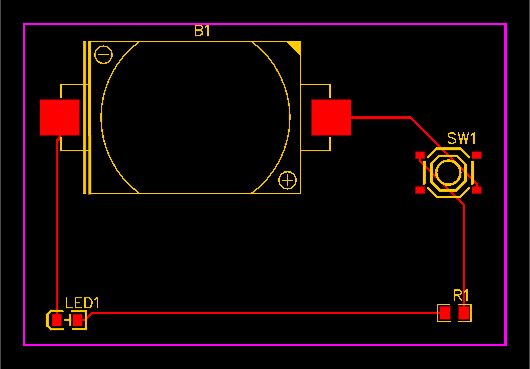
\includegraphics[width=0.8\textwidth]{figures/PCB_PCB_Magisterka_2_2026-11-15}
\caption{Płytka z~diodą LED poprowadzona autorouterem EasyEDA. Źródło:
opracowanie własne.}\label{rys:led-easyeda}
\end{figure}

Autorouter EasyEDA poprowadził wszystkie cztery sieci wyłącznie na warstwie
górnej, bez użycia przelotek. Łączna długość ścieżek wynosi 98,44~mm.
Ścieżki składają się z~odcinków poziomych, pionowych i~nachylonych pod kątem
45°, a~każde połączenie ma tylko kilka załamań. Sprawdzenie reguł
projektowych (DRC) nie wykazało naruszeń.

\begin{figure}[H]
\centering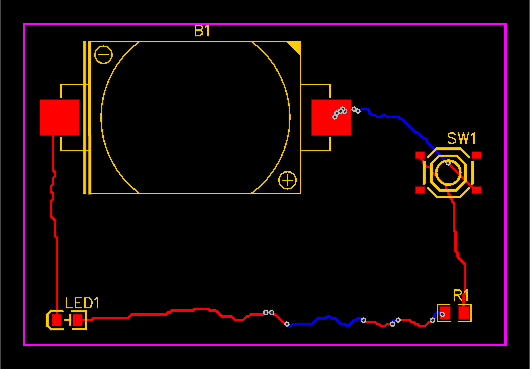
\includegraphics[width=0.8\textwidth]{figures/PCB_PCB_Magisterka_3_2026-11-15}
\caption{Płytka z~diodą LED poprowadzona algorytmem A* bez sieci neuronowej.
Źródło: opracowanie własne.}\label{rys:led-astar}
\end{figure}

Algorytm A* również poprowadził wszystkie cztery sieci, a~DRC nie wykazało
naruszeń reguł projektowych. Łączna długość ścieżek wynosi 106,79~mm, czyli
o~8,5\% więcej niż w~wariancie EasyEDA. Ścieżki wielokrotnie przechodzą
między warstwami, co dało 16~przelotek wobec braku przelotek w~wariancie
EasyEDA. Przebieg ścieżek jest nieregularny: na trasie występuje wiele
drobnych załamań, wynikających z~prowadzenia ścieżek po siatce o~boku
8~mil z~ruchami po przekątnej. Trasowanie trwało 15,0~s, a~algorytm
rozwinął 121\,772~węzły.

\begin{figure}[H]
\centering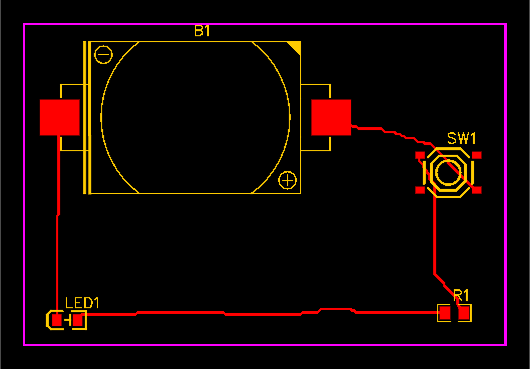
\includegraphics[width=0.8\textwidth]{figures/PCB_PCB_Magisterka_UnetAstar_2026-11-16}
\caption{Płytka z~diodą LED poprowadzona algorytmem Unet-A*. Źródło:
opracowanie własne.}\label{rys:led-unet}
\end{figure}

Algorytm Unet-A* poprowadził wszystkie cztery sieci wyłącznie na warstwie
górnej, bez użycia przelotek, a~DRC nie wykazało naruszeń reguł
projektowych. Łączna długość ścieżek wynosi 100,02~mm. Jest to o~1,6\% więcej
niż w~wariancie EasyEDA i~o~6,3\% mniej niż w~wariancie A*. Przebieg
połączeń jest niemal taki sam jak w~wariancie EasyEDA
(rys.~\ref{rys:led-easyeda}): ścieżki biegną tą samą drogą od gniazda baterii
przez diodę, rezystor i~przycisk. Różnią się jednak kształtem. Zamiast
prostych odcinków mają drobne, schodkowe załamania wynikające z~prowadzenia
po siatce, choć jest ich mniej niż w~wariancie A*.
Trasowanie trwało 4,6~s, czyli ponad trzykrotnie krócej niż w~wariancie A*.
Algorytm rozwinął 61\,582~węzły, o~49\% mniej niż A*.

\begin{table}[ht]
\fcmtcaption{Parametry płytki z~diodą LED w~badanych wariantach. Źródło:
opracowanie własne.}\label{tab:wyniki-led}
\centering\footnotesize%
\begin{tabular}{l r r r}
\toprule
Miara & EasyEDA & A* & Unet-A* \\
\midrule
Połączone sieci & 4/4 & 4/4 & 4/4 \\
\midrule
Długość ścieżek [mm] & 98,44 & 106,79 & 100,02 \\
\midrule
Liczba przelotek & 0 & 16 & 0 \\
\midrule
Naruszenia DRC & 0 & 0 & 0 \\
\midrule
Czas trasowania [s] & --- & 15,0 & 4,6 \\
\midrule
Rozwinięte węzły & --- & 121\,772 & 61\,582 \\
\bottomrule
\end{tabular}
\end{table}

\section{Płytka przykładowa EasyEDA}
\label{sec:wyniki-sample}

Druga płytka testowa pochodzi z~przykładowego projektu (\emph{Sample Project})
udostępnionego w~sekcji \emph{Modules} serwisu
EasyEDA~\cite{EasyEDA_ProjectSample}. Zawiera osiem elementów:
złącze (U1), dwa tranzystory (Q1, Q2), kondensator (C1) i~cztery rezystory
(R1--R4). Elementy mają łącznie 29~padów, z~czego 18~to pady powierzchniowe
(SMD), a~11~pady przewlekane (THT). Płytka ma wymiary $37 \times 25$~mm
i~dwie warstwy sygnałowe. Projekt zawiera sześć sieci.

Wyniki trasowania przedstawiono na
rysunkach~\ref{rys:sample-easyeda}--\ref{rys:sample-unet}, a~ich parametry
zestawiono w~tabeli~\ref{tab:wyniki-sample}.

\begin{figure}[H]
\centering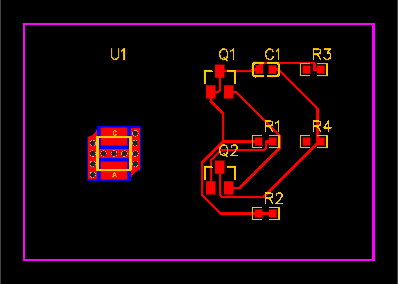
\includegraphics[width=0.8\textwidth]{figures/PCB_PCB_SamplePCB_2026-11-15}
\caption{Płytka przykładowa EasyEDA poprowadzona autorouterem EasyEDA.
Źródło: opracowanie własne.}\label{rys:sample-easyeda}
\end{figure}

Autorouter EasyEDA poprowadził cztery z~sześciu sieci. Niepoprowadzone
pozostały połączenia złącza U1 z~resztą układu. Wszystkie ścieżki leżą na
warstwie górnej, bez przelotek, a~ich łączna długość wynosi 92,51~mm.
DRC wykazało dwa naruszenia reguł projektowych. Oba dotyczą
niedokończonych połączeń, czyli dwóch sieci, których autorouter nie
poprowadził.

\begin{figure}[H]
\centering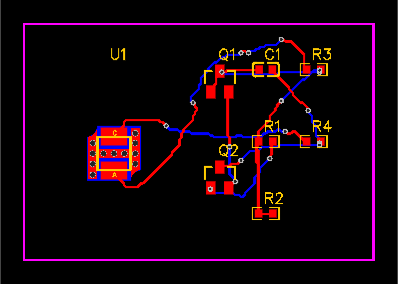
\includegraphics[width=0.8\textwidth]{figures/PCB_PCB_SamplePCB_2026-11-15_2}
\caption{Płytka przykładowa EasyEDA poprowadzona algorytmem A* bez sieci
neuronowej. Źródło: opracowanie własne.}\label{rys:sample-astar}
\end{figure}

Algorytm A* poprowadził wszystkie sześć sieci, łącznie z~połączeniami
złącza U1, a~DRC nie wykazało naruszeń reguł projektowych. Ścieżki
prowadzone są na obu warstwach, co wymagało 18~przelotek. Łączna długość
ścieżek wynosi 149,29~mm, czyli o~61\% więcej niż w~wariancie EasyEDA.
Długości nie są jednak w~pełni porównywalne, ponieważ wariant EasyEDA nie
zawiera dwóch niepoprowadzonych sieci. Podobnie jak na płytce z~diodą LED,
ścieżki mają nieregularny przebieg z~wieloma drobnymi załamaniami.

\begin{figure}[H]
\centering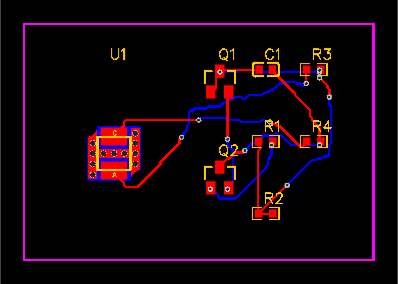
\includegraphics[width=0.8\textwidth]{figures/PCB_PCB_SamplePCB_UnetAstar_2026-11-16}
\caption{Płytka przykładowa EasyEDA poprowadzona algorytmem Unet-A*.
Źródło: opracowanie własne.}\label{rys:sample-unet}
\end{figure}

Algorytm Unet-A* również poprowadził wszystkie sześć sieci, łącznie
z~połączeniami złącza U1. DRC nie wykazało naruszeń reguł projektowych.
Ścieżki prowadzone są na obu warstwach, co wymagało 16~przelotek, o~dwie
mniej niż w~wariancie A*. Łączna długość ścieżek wynosi 146,44~mm. Jest to
o~1,9\% mniej niż w~wariancie A*, ale o~58\% więcej niż w~wariancie EasyEDA.
Tę ostatnią różnicę należy jednak interpretować ostrożnie, ponieważ wariant
EasyEDA nie zawiera dwóch sieci. Kształt ścieżek jest podobny jak
w~wariancie A*: występują drobne załamania wynikające z~prowadzenia po
siatce. Trasowanie trwało 3,1~s wobec 16,6~s dla A*, a~liczba rozwiniętych
węzłów spadła ze 160\,493 do 45\,516, czyli o~72\%.

\begin{table}[ht]
\fcmtcaption{Parametry płytki przykładowej EasyEDA w~badanych wariantach.
Źródło: opracowanie własne.}\label{tab:wyniki-sample}
\centering\footnotesize%
\begin{tabular}{l r r r}
\toprule
Miara & EasyEDA & A* & Unet-A* \\
\midrule
Połączone sieci & 4/6 & 6/6 & 6/6 \\
\midrule
Długość ścieżek [mm] & 92,51 & 149,29 & 146,44 \\
\midrule
Liczba przelotek & 0 & 18 & 16 \\
\midrule
Naruszenia DRC & 2 & 0 & 0 \\
\midrule
Czas trasowania [s] & --- & 16,6 & 3,1 \\
\midrule
Rozwinięte węzły & --- & 160\,493 & 45\,516 \\
\bottomrule
\end{tabular}
\end{table}

\chapter{Wnioski}
\label{ch:wnioski}

\section{Skuteczność trasowania}

Dla większości płytek rozwiązania wyznaczone algorytmami \emph{A*}
i~\emph{Unet-Astar} były gorsze od wyników autoroutera dostępnego w~edytorze
\emph{EasyEDA}. Ze względu na postać funkcji celu bazowa wersja algorytmu
\emph{A*} umieszczała na płytce wiele przelotek. Wersja wspomagana siecią
neuronową w~dużej mierze wyeliminowała ten problem. Ze względu na sposób
modelowania problemu nadal jednak proponowała ścieżki z~wieloma
załamaniami, co zwiększało ich łączną długość. Widoczne są też skutki
zaokrąglania reguł projektowych do oczek siatki. W~niektórych miejscach
algorytm \emph{A*} nie był w~stanie poprowadzić ścieżki, podczas gdy
wbudowany autorouter radził sobie z~tym bez trudu.

Badania wykazały jednak, że zdarzają się przypadki, w~których autorouter
nie poprowadził wszystkich połączeń, a~algorytm \emph{A*} --- zarówno
w~wersji podstawowej, jak i~z~obszarami rekomendowanymi wyznaczanymi przez
sieć konwolucyjną --- poprowadził je w~całości.

\section{Czas trasowania}

Przeprowadzony eksperyment wykazał, że wyznaczanie obszarów rekomendowanych
przez konwolucyjną sieć neuronową znacznie przyspiesza trasowanie
w~porównaniu z~samym algorytmem \emph{A*}. \emph{EasyEDA} nie podaje
wprost czasu trasowania, jednak jest on rzędu kilku sekund, a~więc zbliżony
do czasu działania \emph{Unet-Astar}. Czasów tych nie można jednak
bezpośrednio porównać, ponieważ edytor działający w~przeglądarce wykonuje
obliczenia w~chmurze.

\section{Kierunki dalszych prac w~zakresie trasowania}

W~obecnej implementacji \emph{Unet-Astar} nie stanowi jeszcze
pełnowartościowej alternatywy dla autoroutera \emph{EasyEDA}. Uzyskane
wyniki wskazują jednak, że rozwiązania oparte na sztucznej inteligencji mają
potencjał, by w~przyszłości dorównać klasycznym metodom heurystycznym,
a~nawet je wyprzedzić.

Przewidywanie obszarów rekomendowanych przez sieć konwolucyjną okazało się
korzystne nie tylko pod względem czasu działania, lecz także jakości
wyników. Naturalnym rozwinięciem tej metody byłoby wykorzystanie jako
danych uczących ścieżek wyznaczonych algorytmem \emph{A*} zamiast obszarów
wyznaczanych algorytmem Lee.

Dalszego rozwoju wymaga również implementacja algorytmu \emph{A*}
wykorzystana w~programie. Należy przede wszystkim zmodyfikować funkcję celu
i~systematycznie zbadać wpływ parametrów na wynik algorytmu. Szczególną
uwagę warto zwrócić na zwiększenie kary za nieregularny kształt ścieżki.

% Wygodny format eksportu danych z~narzędzia bardzo ułatwia integrację z~różnymi solverami.
% Dobrym kierunkiem ułatwiającym dalsze prace byłaby automatyzacja importu.
% TODO: podsumowanie i interpretacja wyników, odniesienie do celu pracy, kierunki dalszych prac.


\chapter{Zakończenie}

Celem pracy było zbadanie skuteczności rozwiązań sztucznej inteligencji
w~projektowaniu płytek PCB, na przykładzie trasowania połączeń
i~rozmieszczania elementów. Przeprowadzone eksperymenty pokazują, że
projektowanie złożonych płytek drukowanych pozostanie na razie w~rękach
inżynierów. W~przypadku trasowania wkrótce może jednak nadejść moment,
w~którym wspieranie się sztuczną inteligencją przy wyznaczaniu ścieżek
stanie się codziennością. Sieć neuronowa już teraz wyraźnie przyspiesza
wyszukiwanie ścieżek, choć ich jakość nie dorównuje jeszcze klasycznemu
autorouterowi. W~przypadku rozmieszczania elementów upłynie natomiast
znacznie więcej czasu, zanim doświadczenie i~wiedza projektanta ustąpią
miejsca sztucznej inteligencji.

Nie oznacza to, że temat powinien przestać interesować środowisko
naukowe. Praca stanowi solidną podstawę do dalszych badań, a~kierunków
ich rozwoju jest wiele. Można nawet podjąć próbę wykorzystania dużych
modeli językowych, ponieważ projekty płytek zapisywane są w~formatach
tekstowych, takich jak pliki KiCad czy Specctra DSN. Na dzień dzisiejszy
pytanie o~skuteczność sztucznej inteligencji w~projektowaniu płytek PCB
pozostaje więc otwarte.


%--------------------------------------
% Literatura
%--------------------------------------

\bibliographystyle{plain}{\raggedright\sloppy\small\bibliography{bibliografia}}

%--------------------------------------
% Dodatki
%--------------------------------------

%\cleardoublepage\appendix%
%\newpage
%
\chapter{Składanie dokumentu w systemie \LaTeX}

W tym rozdziale znajduje się
garść informacji o tym, jak poprawnie składać tekst pracy w systemie \LaTeX{} wraz z 
przykładami, które mają służyć do przeklejania do własnych dokumentów.

\section{Struktura dokumentu}
\chaptermark{Tytuł rozdziału, jeśli pełen się nie mieści\ldots{}}{}

Praca składa się z rozdziałów (\texttt{chapter}) i podrozdziałów (\texttt{section}).
Ewentualnie można również rozdziały zagnieżdzać (\texttt{subsection}, \texttt{subsubsection}),
jednak nie powinno się wykraczać poza drugi poziom hierarchii (czyli \texttt{subsubsection}).

\section{Akapity i znaki specjalne}

Akapity rozdziela się od siebie przynajmniej jedną pustą linią. Podstawowe
instrukcje, które się przydają to \emph{wyróżnienie pewnych słów}. Można również
stosować \textbf{styl pogrubiony}, choć nie jest to generalnie zalecane.

Należy pamiętać o zasadach polskiej interpunkcji i ortografii. Po spójnikach 
jednoliterowych warto wstawić znak tyldy ($\sim$), który jest tak zwaną
,,twardą spacją'' i powoduje, że wyrazy nią połączone nie będą rozdzielane
na dwie linie tekstu.

Polskie znaki interpunkcyjne różnią się nieco od angielskich: to jest ,,polski'', a to jest
``angielski''. W kodzie źródłowym tego tekstu będzie widać różnicę.

Proszę również zwrócić uwagę na znak myślnika, który może być pauzą ,,---'' lub
półpauzą: ,,--''. Należy stosować je konsekwentnie. Do łączenia wyrazów używamy
zwykłego ,,-'' (\emph{północno-wschodni}), do myślników --- pauzy lub półpauzy.
Inne zasady interpunkcji i typografii można znaleźć w słownikach.

Przegląd literatury naświetlający stan wiedzy na dany temat obejmuje rozdziały pisane na podstawie
literatury, której wykaz zamieszczany jest w części pracy pt.~\emph{Literatura} (lub inaczej \emph{Bibliografia},
\emph{Piśmiennictwo}). W tekście pracy muszą wystąpić odwołania do wszystkich pozycji zamieszczonych w
wykazie literatury. \textbf{Nie należy odnośników do literatury umieszczać w stopce strony.} Student jest
bezwzględnie zobowiązany do wskazywania źródeł pochodzenia informacji przedstawianych w pracy,
dotyczy to również rysunków, tabel, fragmentów kodu źródłowego programów itd. Należy także podać
adresy stron internetowych w przypadku źródeł pochodzących z Internetu.

Zakończenie pracy zwane również Uwagami końcowymi lub Podsumowaniem powinno zawierać ustosunkowanie
się autora do zadań wskazanych we wstępie do pracy, a w szczególności do celu i zakresu pracy oraz
porównanie ich z faktycznymi wynikami pracy. Podejście takie umożliwia jasne określenie stopnia
realizacji założonych celów oraz zwrócenie uwagi na wyniki osiągnięte przez autora w ramach jego
samodzielnej pracy.

Integralną częścią pracy są również dodatki, aneksy i załączniki zawierające stworzone w ramach pracy programy, aplikacje i projekty.



\section{Wypunktowania}

Wypunktowanie z cyframi:
\begin{enumerate}
    \item to jest punkt,
    \item i to jest punkt,
    \item a to jest ostatni punkt.
\end{enumerate}

\noindent
Po wypunktowaniach czasem nie warto wstawiać wcięcia akapitowego. Wtedy przydatne jest
polecenie \texttt{noindent}. Wypunktowanie z kropkami (tzw.~\emph{bullet list}) wygląda tak:
\begin{itemize}
    \item to jest punkt,
    \item i to jest punkt,
    \item a to jest ostatni punkt.
\end{itemize}

\noindent
Wypunktowania opisowe właściwie niewiele się różnią:
\begin{description}
    \item[elementA] to jest opis,
    \item[elementB] i to jest opis,
    \item[elementC] a to jest ostatni opis.
\end{description}


\section{Polecenia pakietu \texttt{ppfcmthesis}}

Parę poleceń zostało zdefiniowanych aby uspójnić styl pracy. Są one przedstawione poniżej
(oczywiście nie trzeba się do nich stosować).

\paragraph{Makra zdefiniowane dla języka angielskiego.} Są nimi: \texttt{termdef} oraz \texttt{acronym}.
Przykłady poniżej obrazują ich przewidywane użycie w tekście.
\begin{center}\footnotesize%
\begin{tabular}{l >{\rightskip\fill}p{12cm}}
\toprule
źródło   & \texttt{we call this a $\backslash$termdef\{Database Management System\} ($\backslash$acronym\{DBMS\})} \\ \cmidrule(lr){2-2}
docelowo & we call this a \termdef{Database Management System} (\acronym{DBMS}) \\ 
\bottomrule
\end{tabular}
\end{center}

\paragraph{Makra zdefiniowane dla języka polskiego.} Podobnie jak dla języka angielskiego zdefiniowano
odpowiedniki polskie: \texttt{defini\-cja}, \texttt{akronim} oraz \texttt{english} dla tłumaczeń angielskich
terminów. Przykłady poniżej obrazują ich przewidywane użycie w tekście.
\begin{center}\footnotesize%
\begin{tabular}{l >{\rightskip\fill}p{12cm}}
\toprule
źródło   & \texttt{nazywamy go $\backslash$definicja\{systemem zarządzania bazą danych\} ($\backslash$akronim\{DBMS\}, $\backslash$english\{Database Management System\})} \\ \cmidrule(lr){2-2}
docelowo & nazywamy go \definicja{systemem zarządzania bazą danych} (\akronim{DBMS}, \english{Database Management System}) \\ \bottomrule
\end{tabular}
\end{center}


\section{Rysunki}

Wszystkie rysunki (w tym również diagramy, szkice i inne) osadzamy w środowisku 
\texttt{figure} i umieszczamy podpis \emph{pod} rysunkiem, w formie elementu \texttt{caption}. Rysunki powinny
zostać umieszczone u góry strony (osadzone bezpośrednio w treści strony zwykle utrudniają czytanie tekstu).
Rysunek~\ref{rys:plama} zawiera przykład pełnego osadzenia rysunku na stronie.

\begin{figure}[t] % możliwe opcje to 't' - top, 'b' - bottom, 'h' - 'here', ale zaleca się 't'
\centering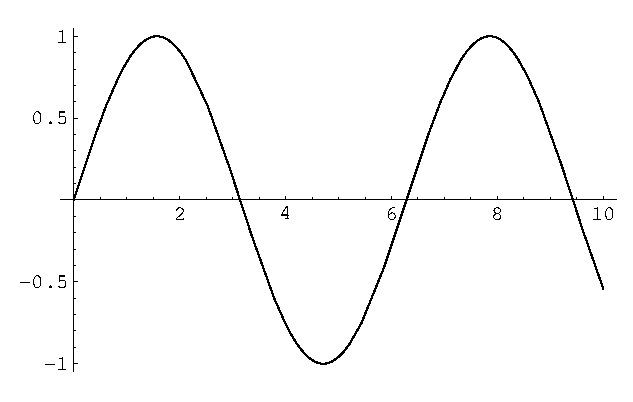
\includegraphics[width=5cm]{figures/mathematica}
\caption{Wykres.}\label{rys:plama}
\end{figure}

\begin{figure}[t]
\centering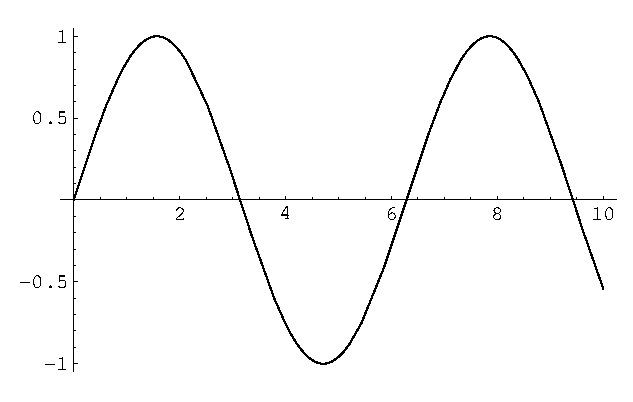
\includegraphics[width=\textwidth]{figures/mathematica}
\fcmfcaption{Ten sam wykres ale na szerokość tekstu. Formatowanie podpisu zgodne z wytycznymi FCMu.}\label{rys:plama2}
\end{figure}

Styl FCMu to nieco inne nagłówki rysunków. Dostepne są one poleceniem \texttt{fcmfcaption} (zob.~rysunek
\ref{rys:plama2}).

\subsection{Tablice}

Tablice to piękna rzecz, choć akurat ich umiejętne tworzenie w \LaTeX{}u nie jest łatwe. 
Jeśli tablica jest skomplikowana, to można ją na przykład wykonać w programie
OpenOffice, a następnie wyeksportować jako plik \akronim{PDF}. W każdym przypadku tablice wstawia się podobnie
jak rysunki, tylko że w środowisko \texttt{table}. Tradycja typograficzna sugeruje umieszczenie opisu tablicy, a więc
elementu \texttt{caption} ponad jej treścią (inaczej niż przy rysunkach).  

Tablica~\ref{tab:tabela} pokazuje pełen przykład.

\begin{table}[ht]
\caption{Przykładowa tabela. Styl opisu jest zgodny z rysunkami.}\label{tab:tabela}
\centering\footnotesize%
\begin{tabular}{l c}
\toprule
artykuł & cena [zł] \\
\midrule
bułka   & $0,4$ \\
masło   & $2,5$ \\
\bottomrule
\end{tabular}
\end{table}

Zasady FCMu sugerują nieco inne nagłówki tablic. Dostepne są one poleceniem \texttt{fcmtcaption} (zob.~tablicę
\ref{tab:tabela2}).

\begin{table}[ht]
\fcmtcaption{Przykładowa tabela. Styl opisu jest zgodny z wytycznymi FCMu.}\label{tab:tabela2}
\centering\footnotesize%
\begin{tabular}{l c}
\toprule
artykuł & cena [zł] \\
\midrule
bułka   & $0,4$ \\
masło   & $2,5$ \\
\bottomrule
\end{tabular}
\end{table}


\subsection{Checklista}

\begin{itemize}
\item Znakiem myślnika jest w LaTeXu dywiz pełen (---) albo półpauza (--), przykład:
  A niech to jasna cholera --- wrzasnąłem.

\item Połączenie między wyrazami to zwykły myślnik, przykład:   północno-zachodni

\item Sprawdź czy tutuł pracy ma maksymalnie dwa wiersze i czy stanowią one pełne frazy
  (czy nie ma przeniesienia bez sensu).

\item Sprawdź ostrzeżenia o 'overfull' i 'underful' boxes. Niektóre z nich można zignorować (spójrz
  na wynik formatowania), niektóre trzeba poprawić; czasem przeformułować zdanie.

item Przypisy stawia się wewnątrz zdań lub za kropką, przykład:
  Footnote is added after a comma.\footnote{Here is a footnote.}

\item Nie używaj przypisów zbyt często. Zobacz, czy nie lepiej będzie zintegrować przypis z tekstem.

\item Tytuły tabel, rysunków powinny kończyć się kropką.

\item Nie używaj modyfikatora [h] (here) do rysunków i tabel. Rysunki i tabele powinny być
  justowane do góry strony lub na stronie osobnej.

\item Wyróżnienie w tekście to polecenie \emph{wyraz}, nie należy używać czcionki pogrubionej (która
  wystaje wizualnie z tekstu i rozprasza).

\item Nazwy plików, katalogów, ścieżek, zmiennych środowiskowych, klas i metod formatujemy poleceniem
  \texttt{plik\_o\_pewnej\_nazwie}.

\item Po ostatniej zmianie do treści, sprawdź i przenieś wiszące spójniki wstawiając przed nie znak
  tyldy (twardej spacji), przykład:
  Ala i~kotek nie lubią mleczka, a~Stasiu lubi.
  
\item Za i.e. (id est) i e.g. (exempli gratia) stawia się zwyczajowo przecinek w typografii amerykańskiej.

\item Przed i za pełną pauza nie ma zwyczajowo spacji w typografii amerykańskiej, przykład:
  Darn, this looks good---said Mary.

\item Zamykający cudzysłów oraz footnote wychodzą za ostatni znak interpunkcji w typografii 
  amerykańskiej, przykłady:
  It can be called a ``curiosity,'' but it's actually normal.
  Footnote is added after a comma.\footnote{Here is a footnote.}

\item Odwołania do tabel i rysunków zawsze z wielkiej litery, przykład:
  In Figure~\ref{rys:plama} we illustrated XXX and in Table~\ref{tab:tabela} we show detailed data.
  
\end{itemize}


\section{Literatura i materiały dodatkowe}

Materiałów jest mnóstwo. Oto parę z nich:
\begin{itemize}
    \item \emph{The Not So Short Introduction\ldots}, która posiada również tłumaczenie 
    w języku polskim.\\
    \url{http://www.ctan.org/tex-archive/info/lshort/english/lshort.pdf}

    \item Klasy stylu \texttt{memoir} posiadają bardzo wiele informacji o składzie tekstów
    anglosaskich oraz sposoby dostosowania \LaTeX{}a do własnych potrzeb.\\
    \url{http://www.ctan.org/tex-archive/macros/latex/contrib/memoir/memman.pdf}
    
    \item Nasza grupa dyskusyjna i repozytorium Git są również dobrym miejscem aby zapytać
    (lub sprawdzić czy pytanie nie zostało już zadane).\\
    \url{https://github.com/politechnika/put-latex}

    \item Dla łaknących więcej wiedzy o systemie LaTeX podstawowym źródłem informacji
    jest książka Lamporta~\cite{Lamport1985}. Prawdziwy \emph{hardcore} to oczywiście
    \emph{The \TeX{}book} profesora Knutha~\cite{Knuth1986}.
\end{itemize}



%--------------------------------------
% Informacja o prawach autorskich
%--------------------------------------

\ppcolophon

\end{document}
